\section{Theorie}
\label{sec:Theorie}

\subsection{Gedämpfte Schwingung}
    Werden in einem Stromkreis zwei Energiespeicher in Form einer Kapazität C
    und einer Induktivität L eingebaut, so kann ein hereingepumpter Energiebetrag
    zwischen beiden hin- und her pendeln. \\
    Da die Energie durch kein Element verbraucht wird, ist sie erhalten.
    Es handelt sich daher um eine ungedämpfte Schwingung.\\

    \noindent Nun kann aber wie in Abbildung \ref{fig:ung}
    dargestellt ein ohmscher Widerstand eingebaut werden, der dem System 
    Energie entzieht. Die Amplituden der Stromes und der Spannung am Kondensator
    nehmen also mit der Zeit ab, es handelt sich um eine gedämpfte Schwingung.\\

    \begin{figure}
        \centering
        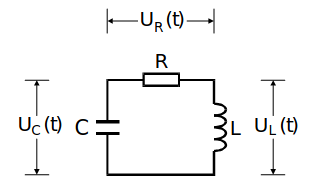
\includegraphics[width=0.5\textwidth]{RLC.png}
        \caption{Gedämpfter Schwinkreis schematisch dargestellt.\cite{anleitung}}
        \label{fig:ung}
    \end{figure}

    \noindent Zur genaueren Beschreibung des periodischen Vorgangs ist 
    das Lösen einer Differentialgleichung nötig, die aus dem 2. Kirchhoffschen 
    Gesetz folgt. Es gilt demnach
    \begin{equation}
        U_R(t) + U_C(t) + U_L(t) = 0
        \label{eqn:kirch}
    \end{equation}
    
    \noindent Zudem gelten das Ohm'sche Gesetz $U_R(t) = R I(t)$ und
    das Induktionsgesetz $U_L(t) = L \frac{\symup{dI}}{\symup{dt}}$, sowie,
    mit der Kondensatorladung Q, $U_C(t) = \frac{Q(t)}{C}$.
    Nach Einsetzen folgt also aus \eqref{eqn:kirch}
    
    \begin{equation*}
        L \frac{\symup{dI}}{\symup{dt}} + R I + \frac{Q(t)}{C} = 0
    \end{equation*}
    
    \noindent Da der Strom auch als Ableitung der Ladung geschrieben werden
    kann, folgt insgesamt die lineare, homogene Differentialgleichung
    
    \begin{equation}
        \frac{d^2 I}{\text{dt}^2} + \frac{R}{L} \frac{dI}{\text{dt}}
        + \frac{1}{LC} I = 0
        \label{eqn:dif1}
    \end{equation}
    
    \noindent Es wird ein Exponentialansatz $I(t) = A \exp(i \omega t)$ 
    gewählt. Nach Ableiten und Einsetzen in \eqref{eqn:dif1} ergibt sich

    \begin{align*}
        \left( -\omega^2 + i \frac{R}{L} \omega + \frac{1}{LC}\right) \cdot A \exp(i \omega t) = 0\\
        \implies \omega^2 - i \frac{R}{L} \omega - \frac{1}{LC} = 0\\
        \implies \omega_{1/2} = i \frac{R}{2L} \pm \sqrt{\frac{1}{LC} - \frac{R^2}{4L^2}}
    \end{align*}

    \noindent Die Gesamtlösung ist eine Superposition der einzelnen Lösungen
    mit 

    \begin{equation*}
        I(t) = A_1 e^{i \omega_1 t} + A_2 e^{i \omega_2 t}
    \end{equation*}

    \noindent Um die Funktion übersichtlich darstellen zu können, seien
    $2 \pi \mu = \frac{R}{2L}$ und $2 \pi \nu = \sqrt{\frac{1}{LC} - \frac{R^2}{4L^2}}$. 
    Dann wird sie zu 

    \begin{equation*}
        I(t) = e^{-2 \pi \mu} \left( A_1 e^{i 2 \pi \nu t} + A_2 e^{-i 2 \pi \nu t}\right)
    \end{equation*}

    \noindent In der weiteren Betrachtung muss nun zwischen verschiedenen
    Verhältnissen von $\frac{1}{RC}$ und $\frac{R^2}{4L^2}$ unterschieden werden.
    je nach dem ist $\nu$ reell oder imaginär. Hier sollen zwei der drei 
    mögliche Fälle betrachtet werden.

    \subsubsection{Schwingfall}
    Zunächst sei
    
    \begin{equation*}
        \frac{1}{RC} > \frac{R^2}{4L^2}
    \end{equation*}
    
    sodass $\nu$ reell ist und die Linearfaktoren
    
    \begin{align*}
        A_1 = \frac{1}{2} A_0 e^{i \eta}\\
        A_2 = \frac{1}{2} A_0 e^{-i \eta}
    \end{align*}

    \noindent Daraus ergibt sich mithilfe der Eulerschen Formel für die Exponentialfunktion
    
    \begin{equation}
        I(t) = A_0 e^{-2 \pi \mu t}  \cos(2 \pi \nu t + \eta)
        \label{eqn:schwingfall}
    \end{equation}

    \noindent Die exponentiell abnehmende Amplitude verschwindet für $t \to \infty$.
    Die Abklingdauer $T_\text{ex} = \frac{2L}{R}$ ist die Zeit, in der die
    Schwingungsdauer auf ein e-tel ihres ursprünglichen Wertes absinkt.
    Abbildung \ref{fig:kurve} zeigt die Schwingung und Einhüllende der des Stromes
    beim Schwingfall.

    \begin{figure}
        \centering
        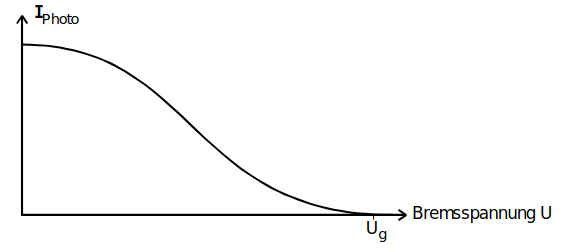
\includegraphics[width=0.5\textwidth]{kurve.png}
        \caption{Strom als Funktion der Zeit beim Schwingfall.\cite{anleitung}}
        \label{fig:kurve}
    \end{figure}

    \subsubsection{Aperioder Grenzfall}
    Beim zweiten Fall, dem aperiodischen Grenzfall, ist $\nu$ rein imaginär,
    da 

    \begin{equation*}
        \frac{1}{LC} < \frac{R^2}{4L^2}
    \end{equation*}

    \noindent Durch die reellen Exponenten schwingt die Funktion nicht mehr, es
    wird von aperiodischer Dämpfung gesprochen. \\
    Nach einiger Zeit gilt
    
    \begin{equation*}
        I \propto \exp \left( - \left( \frac{R}{2L} - \sqrt{ \frac{R^2}{4L^2} - \frac{1}{LC}} \right) t \right)
    \end{equation*}

    Für den Spezialfall, dass $\nu = 0$ ist, gelten

    \begin{equation}
        \frac{1}{LC} = \frac{R^2_{\text{ap}}}{4L^2}
        \label{eqn:spezialfall}
    \end{equation}

    und

    \begin{equation*}
        I(t) = A e^{-\frac{R}{2L}t} = A e^{- \frac{t}{\sqrt{LC}}}
    \end{equation*}

    Der Spezialfall ist in Abbildung \ref{fig:ape} als gestrichelte Linie eingezeichnet. 
    Der Strom geht dabei ohne jegliche Schwingunge gegen null.

    \begin{figure}
        \centering
        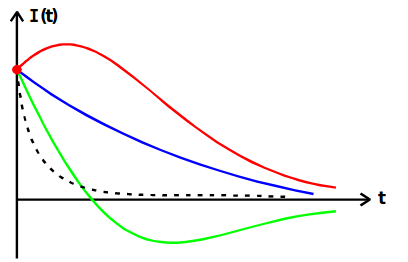
\includegraphics[width=0.5\textwidth]{aperiod.png}
        \caption{Verschiedene Verläufe der aperiodischen Dämpfung.\cite{anleitung}}
        \label{fig:ape}
    \end{figure}

\subsection{Erzwungene Schwingungen}
    Anderes Verhalten zeigt sich beim Anschließen einer äußeren periodischen Kraft,
    in diesem Falle eine Spannungsquelle, die für eine sinusförmige Wechselspannung
    $U(t) = U_0 e^{i \omega t}$
    sorgt. Der Schaltkreis ist in \ref{fig:schwingschwing} zu sehen.

    \begin{figure}
        \centering
        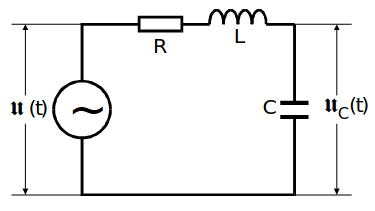
\includegraphics[width=0.5\textwidth]{erzwungen.png}
        \caption{Stromkreis der erzwungenen Schwingung.}
        \label{fig:schwingschwing}
    \end{figure}

    \noindent Dann kommt zur Gleichung \eqref{eqn:kirch} die angelegte Spannung
    als Inhomogenität hinzu und es folgt die Differentialgleichung
    
    \begin{equation}
        LC \frac{d^2 U_C}{\text{dt}^2} + RC \frac{d U_C}{\text{dt}} + U_C = U_0 e^{i \omega t}
        \label{eqn:dif2}
    \end{equation}

    \noindent wobei verwendet wurde, dass $U_C (t) = \frac{Q(t)}{C}$ die Spannung am 
    Kondensator ist und $I = \frac{d U_C}{\text{dt}}$ deren zeitliche Änderung.
    Es wird erneut ein Exponentialansatz verwendet, dessen Amplitude nun aber 
    frequenzabhängig sein kann.

    \begin{equation}
        U_C(\omega, t) = U(\omega) e^{i \omega t}
        \label{eqn:ansatz}
    \end{equation}

    \noindent Nach Einsetzen in \eqref{eqn:dif2} ergibt sich die Funktion
    \begin{equation*}
        U(\omega) = \frac{U_0 \left( 1 - LC \omega^2 - i \omega RC\right)}
        {\left(1 - LC \omega^2\right)^2 + \omega^2 R^2 C^2}
    \end{equation*}
    
    \noindent Deren Betrag ist gegeben durch 
    \begin{equation}
        |U| = U_0 \sqrt{\frac{\left(1 - LC \omega^2\right)^2 + \omega^2 R^2 C^2}
        {\left(\left( 1 - LC \omega^2\right)^2 + \omega^2 R^2 C^2\right)^2}}
    \end{equation}

    \noindent während die Phase sich zu 
    
    \begin{equation}
        \tan \phi = \frac{- \omega R C}{1 - LC \omega^2}\\
        \iff \phi = \text{arc} \tan\left(\frac{- \omega R C}{1-LC \omega^2}\right)
    \end{equation}

    ergibt.\\
    Es muss allerdings von $U_C$ gleich dem Betrag von $U$ sein, wie an \eqref{eqn:dif2}
    zu erkennen ist. So folgt also
    \begin{equation}
        U_C(\omega) = \frac{U_0}{\sqrt{\left(1-LC\omega^2\right)^2 + \omega^2 R^2 C^2}}
        \label{solution}
    \end{equation}

    \noindent Die Grenzfälle sind

    \begin{align*}
        \omega \to \infty \implies U_C \to 0 \\
        \omega \to 0 \implies U_C \to U_0
    \end{align*}

    \noindent Zwischen diesen erreicht die Kondensatorspannung ein Maximum
    bei der sogenannten Resonanzfrequenz. Für die gilt

    \begin{equation}
        \omega_{\text{res}} = \sqrt{\frac{1}{LC} - \frac{R^2}{2L^2}}
        \label{eqn:resonance}
    \end{equation}
    
    \subsubsection{Schwache Dämpfung}
        Für den Fall, dass $\frac{R^2}{2L^2} << \frac{1}{LC}$ wird von schwacher 
        Dämpfung gesprochen. Die Resonanzfrequenz geht gegen die Frequenz 
        der ungedämpften Schwingung und für die Kondensatorspannung folgt
        \begin{equation*}
            U_{C, \text{max}} = \frac{1}{\omega_0 RC} U_0 = \frac{1}{R} \sqrt{\frac{L}{C}} U_0
        \end{equation*}
        \noindent Dabei wird die Güte 
        \begin{equation}
            q = \frac{1}{R} \sqrt{\frac{L}{C}}
            \label{eqn:gute}
        \end{equation}
        definiert. Sie kann auch durch die Frequenzen $\omega_+$, $\omega_-$
        dargestellt werden. $\omega_+$, $\omega_-$ sind die Frequenzen, bei 
        denen für die Spannung gilt $U_C = \frac{1}{\sqrt{2}}U_{C, \text{max}}$.
        Aus der Breite der Resonanzkurve
        \begin{equation}
            \omega_+ - \omega_- \approx \frac{R}{L}
        \end{equation}
        folgt
        \begin{equation*}
            q = \frac{\omega_0}{\omega_+ - \omega_-}
        \end{equation*}

    \subsubsection{Starke Dämpfung}
        Im gegenteiligen Fall gilt $\frac{R^2}{2L^2} >> \frac{1}{LC}$, es liegt
        also starke Dämpfung vor. Die Kondensatorspannung nähert sich monoton
        der null an und geht nicht über $U_0$ hinaus. \\
        Dann ist $U_C \propto \frac{1}{\omega^2}$ für große Frequenzen.

    \subsubsection{Impedanz}
        Interpretiert man den Schwingkreis als Zweipol, so hat er eine komplexe
        Impedanz, die sich aus den Impedanzen der einzelnen Bestandteile zusammensetzt.
        Schematisch ist der Zweipol in Abbildung \ref{fig:zwei} dargestellt.
        \begin{figure}
            \centering
            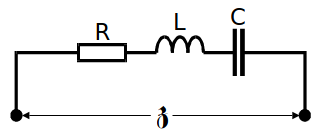
\includegraphics[width=0.5\textwidth]{zweipol.png}
            \caption{Interpretation des Schwingkreises als Zweipol.\cite{anleitung}}
            \label{fig:zwei}
        \end{figure}

        \noindent Die Impedanz kann durch $Z = X + iY$ dargestellt werden. Dabei ist 
        X der Wirkwiderstand und Y der Blindwiderstand. $|Z|$ wird als Scheinwiderstand
        bezeichnet.\\
        Bei Untersuchungen der Impedanz interessiert insbesondere der Verlauf
        in der komplexen Zahlenebene.\\
        Für den Fall des Serienschwingkreises gilt
        \begin{align*}
            Z_C = -\frac{i}{\omega}{C}\\
            Z_L = i \omega L\\
            Z_R = R\\
            \implies Z_{\text{ges}} = R + i\left(\omega L - \frac{1}{\omega C}\right)\\
            \implies |Z_{\text{ges}}| = \sqrt{R^2 + \left(\omega L - \frac{1}{\omega C}\right)^2}
        \end{align*}

        \noindent Der Scheinwiderstand hat also sein Minimum bei $\omega_0 = \frac{1}{\sqrt{LC}}$.
        Dabei ist $|Z_{\text{min}}| = R$, während er sowohl für $\omega \to 0$ als auch
        für $\omega \to \infty$ gegen unendlich geht.
